\chapter{Introduction}
\label{introduction}

\begin{figure}
    \centering
    \begin{subfigure}[b]{0.3\textwidth}
        \label{fig:qft_lo_ee_scattering}
        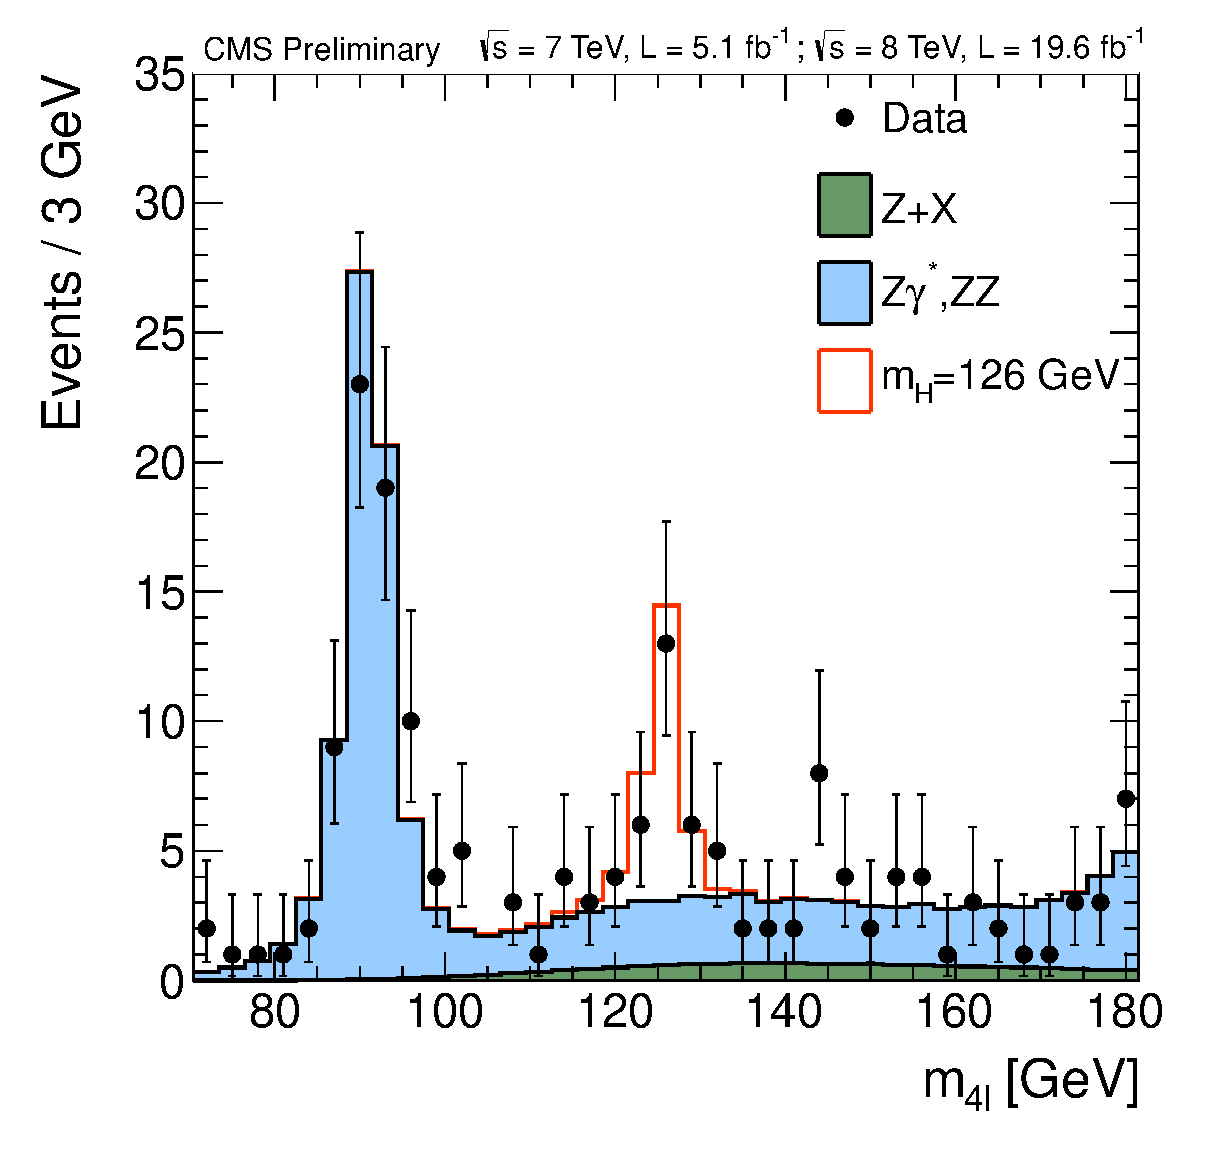
\includegraphics[width=\textwidth]{Figures/Experimental_Results/CmsHZZ4lMass.eps}
        \caption{CMS results for the $H\rightarrow~ZZ$ channel}
      \end{subfigure}
      ~ %add desired spacing between images, e. g. ~, \quad, \qquad, \hfill etc.
      % (or a blank line to force the subfigure onto a new line)
      \begin{subfigure}[b]{0.3\textwidth}
          \label{fig:qft_nlo_ee_scattering}
          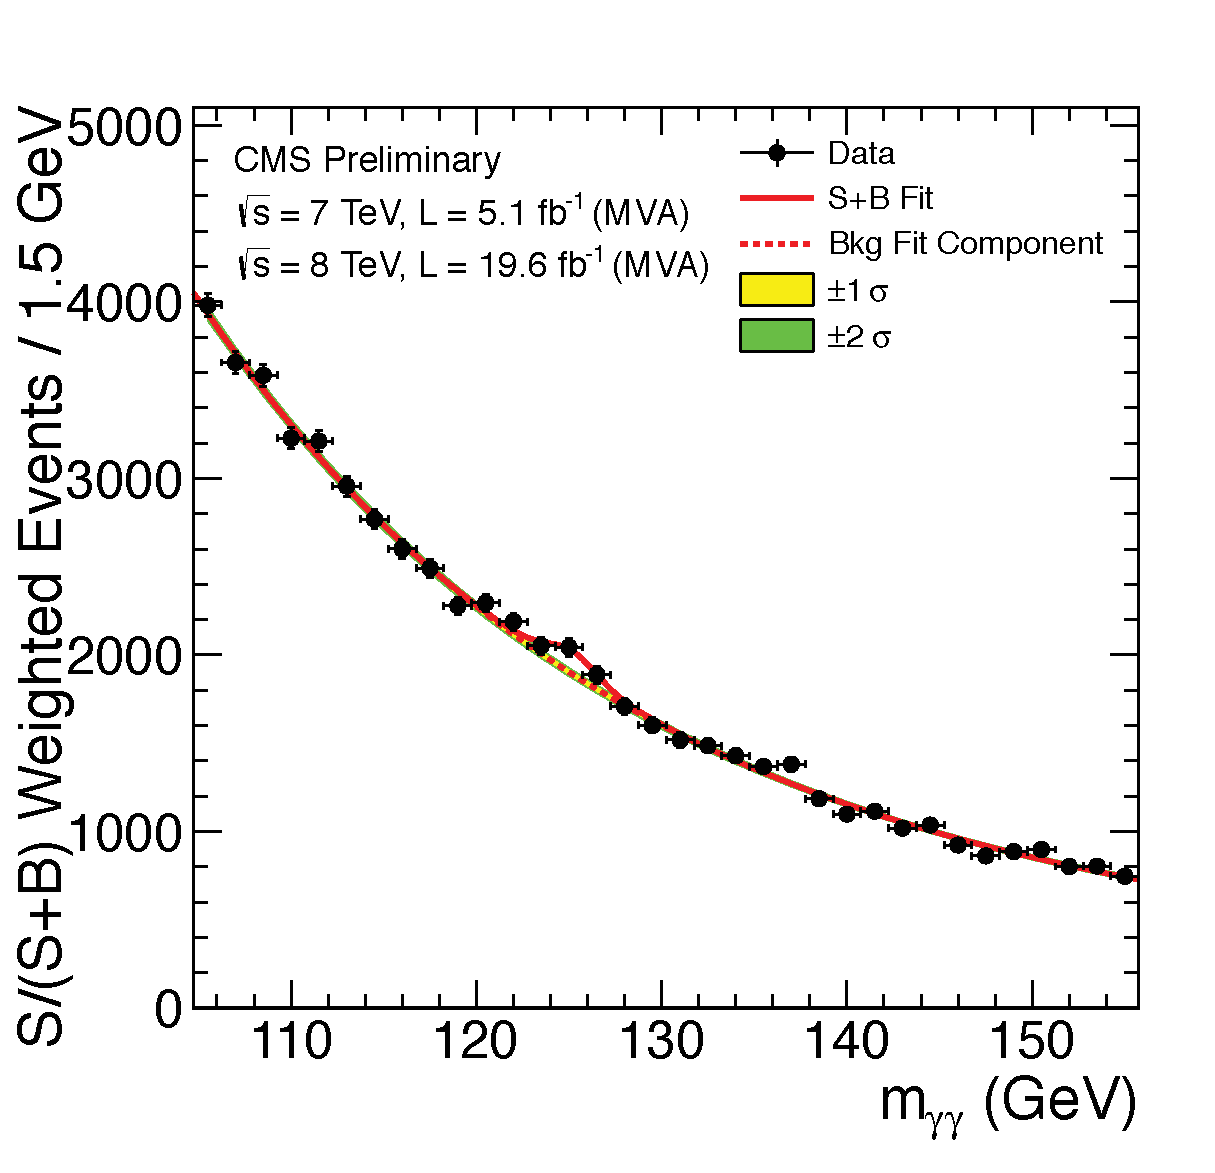
\includegraphics[width=\textwidth]{Figures/Experimental_Results/CmsHggMassMVAMoriond13.eps}
          \caption{CMS results for the $H\rightarrow\gamma\gamma$ channel}
      \end{subfigure}
      \caption{The CMS experiment has observed a new boson at m$\sim$125\GeVcc} \label{fig:cms_hZZ_hgg_results}
\end{figure}

\par On July 4th, 2012, the \acrfull{cms} and \acrfull{atlas} experiments announced the discovery of a new boson of mass $\sim~125$~\GeVcc~\cite{CMS:2012discovery}~\cite{ATLAS:2012discovery}.  The particle has been shown to be increasingly consistent with the description of the boson predicted by the Higgs mechanism of the \acrshort{sm}, as measurements on its mass, width, and quantum numbers are completed.  However, there are several properties of this new boson, which remain to be tested.  Figure \ref{fig:cms_hZZ_hgg_results} shows a consistent mass peak betwen the $H\rightarrow~ZZ$ and $H\rightarrow\gamma\gamma$ channels at the \acrshort{cms} experiment.  

\par The Yukawaka coupling of the Higgs boson to the top-quark in the \acrshort{sm} is the largest coupling among the fundamental particles and is well 
predicted - thus offering an excellent test of the nature of the coupling of the Higgs to fermions, as well as a potential probe into pysics \acrfull{bsm} that would alter this value from the \acrshort{sm} prediction.  The production of the Higgs boson in association with top-quark pairs is the best production mode at the \acrshort{lhc} that offers direct access to the top-Higgs coupling.  The dominant production mode of Higgs at the \acrshort{lhc}, gluon-gluon fusion, involves a triangle loop of strongly-coupled fermions, which includes all of the other quarks, as well as the potential for \acrshort{bsm} particles.  

\par ~\ttH~production also has the ability to constrain some extensions of the \acrshort{sm} that would not modify the Higgs branching fractions enough to be seen 
within current experiemental precision.  Such models include Little Higgs models, models with extra dimensions, top-color models, and composite Higgs models that introduce a vector-like top partner, a $t'$, that can decay to $tH$, $bW$, or $tZ$ states.  Both $t't'$ and $t't$ production would produce a~\ttH~final state, or one that is indistinguishable from it ($tHbW$).  Upper limits on~\ttH~production would also provide limits on the previously described models, which would be complementary to existing direct searches for $t'$ particles, which attempt to reconstruct the $t'$ resonance.  

\par The~\ttH~channel has a rich set of possible final states.  Each top-quark will decay to a $b$-quark and a $W$ boson.  The $W$ boson will subsequently decay to two quarks, or a lepton and a neutrino.  These decays are classified as either hadronic, semi-leptonic, or di-leptonic for zero, one, or both $t$ quarks decaying leptonically 
respectively.  The Higgs may to decay to $b$-quark, $W$, $Z$, $\tau$, or $\gamma$ pairs.  In fact, this is one of the only production modes at the \acrshort{lhc} which 
has access to every Higgs decay mode, as other production mechanisms are swamped by large backgrounds preventing measurements of all Higgs decay types.  

\par The search is performed with the \acrshort{cms} experiment, a modern, general purpose particle detector capable of reconstructing and identifying hadronic jets, photons, electrons, muons, and tau leptons.  The hermetic design, and it's high precision and efficiency in reconstrucing and tracking every particle in a $pp$ collision, also makes it suitable for reconstructing missing transverse energy from the calculated momentum imbalance of all of the measured particles in the event.  This missing transverse energy is often the signature of a neutrino, which is the only \acrshort{sm} particle capable of escaping detection.  The detector uses a 3.8 T axial magnetic field, produced by the solenoid it is named after, to bend charged particles as they travel through the detector.  The measured curvature of their tracks allows the momentum of the particles to be calculated with to a high precision.  Tracks are formed and particles are reconstructed by a combination of sub-detector systems which work together to form the final final reconstructed image of each particle in the collision.  

\begin{figure}[h]
   \centering
  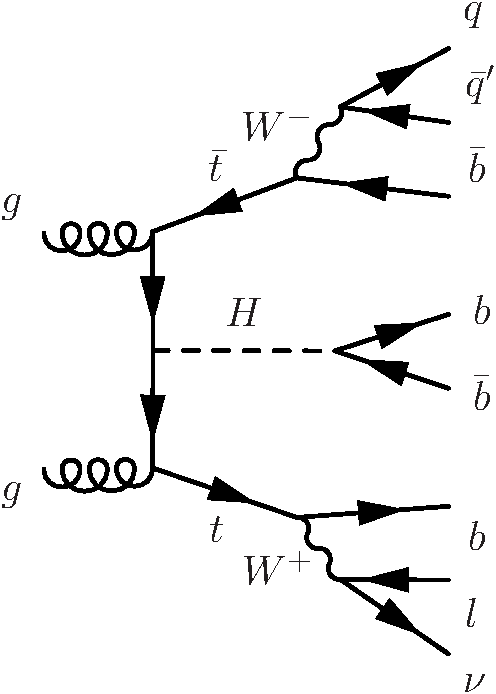
\includegraphics[width=0.5\textwidth]{Figures/Feynman_Diagrams/higgs_production__tth_semileptonic.pdf}
  \caption{A Feynman diagram of the~\ttH~process, with Higgs$\rightarrow$$b\bar{b}$, and the $t\bar{t}$-system decaying semi-leptonically} \label{fd:ttH_semiLep}
\end{figure}

\par This thesis will focus on a semi-leptonic decay of the top-quarks, with the Higgs decaying to a $b$-quark pair.  Figure \ref{fd:ttH_semiLep} is Feynman diagrm of the~\ttH~process.  The largest background to this process is top-quark pair production with extra jets originating from \acrfull{isr} or \acrfull{fsr} radiation,~\ttjets.  The irreducible background is formed by top-quark pairs, where a gluon is radiated and decays to $b$-quark pairs,~\ttbb.  In addition to the large backgrounds, the high jet multiplicity in the~\ttH~final state gives rise to a combinatorics problem in associating each jet with its role in the~\ttH~system.  This inevitably leads to misidentifying which jets are the decay product of the Higgs, and thus additionally smears out the resolution on the mass of the Higgs.  Due to the similarity of the~\ttbb~background and the combinatorics issue, no single variable is suitable for signal extraction.  A \acrfull{mva} technique is used in an attempt to isolate the~\ttH~signal from the~\ttjets background.  The \acrshort{mva} provides a one-dimensional discriminant based on several input variables related to the kinematics of the event.  This discrimant is then used to perform signal extraction and set upper-limits on~\ttH~ production.  The results of two searches will be presented.  The first result used the first 5.1~\fbinv of the 2012 dataset, with center of mass energy of 8~\TeV, and was published in the \acrfull{jhep}, May 2013.  The second result was update with the full 19.4~\fbinv 8~\TeV dataset, and was published in \acrshort{jhep}, Spetember 2014.   
